\documentclass[12pt,a4paper]{article}
\usepackage{physics}
\usepackage{amssymb}
\usepackage{subcaption}
\usepackage{colortbl}
\input{spp.dat}

%  Editorial staff will uncomment the next line
% \providecommand{\artnum}[0]{XX-XX}
% \renewcommand{\articlenum}[0]{SPP-\the\year-\artnum-}

\begin{document}

\title{\TitleFont Activity 3 -- Image Types and Formats}
\author[ ]{\textbf{Kenneth V. Domingo} \\
2015--03116 \\
App Physics 186, 1\textsuperscript{st} Semester, A.Y. 2019--20}
\affil[ ]{\corremail{kvdomingo@up.edu.ph} }

\maketitle
\thispagestyle{titlestyle}

\section*{Results and Discussion}
\setcounter{section}{1}

\subsection{File formats}
The image I used for the comparison of file sizes is an HDR image of the Oblation Plaza overlooking University Avenue during sunset taken by myself, shown in Fig. \ref{fig:hdr}. Its histogram is shown in Fig. \ref{fig:hist}. I've already post-processed the image so that it displays properly on print or on non-HDR-capable devices. The file sizes themselves are shown in Table \ref{tab:sizes}. In the interest of minimizing the size of this submission, I will no longer include the images saved in other file formats if there is no perceivable change in quality/characteristics.

\begin{figure}[htb]
	\centering
	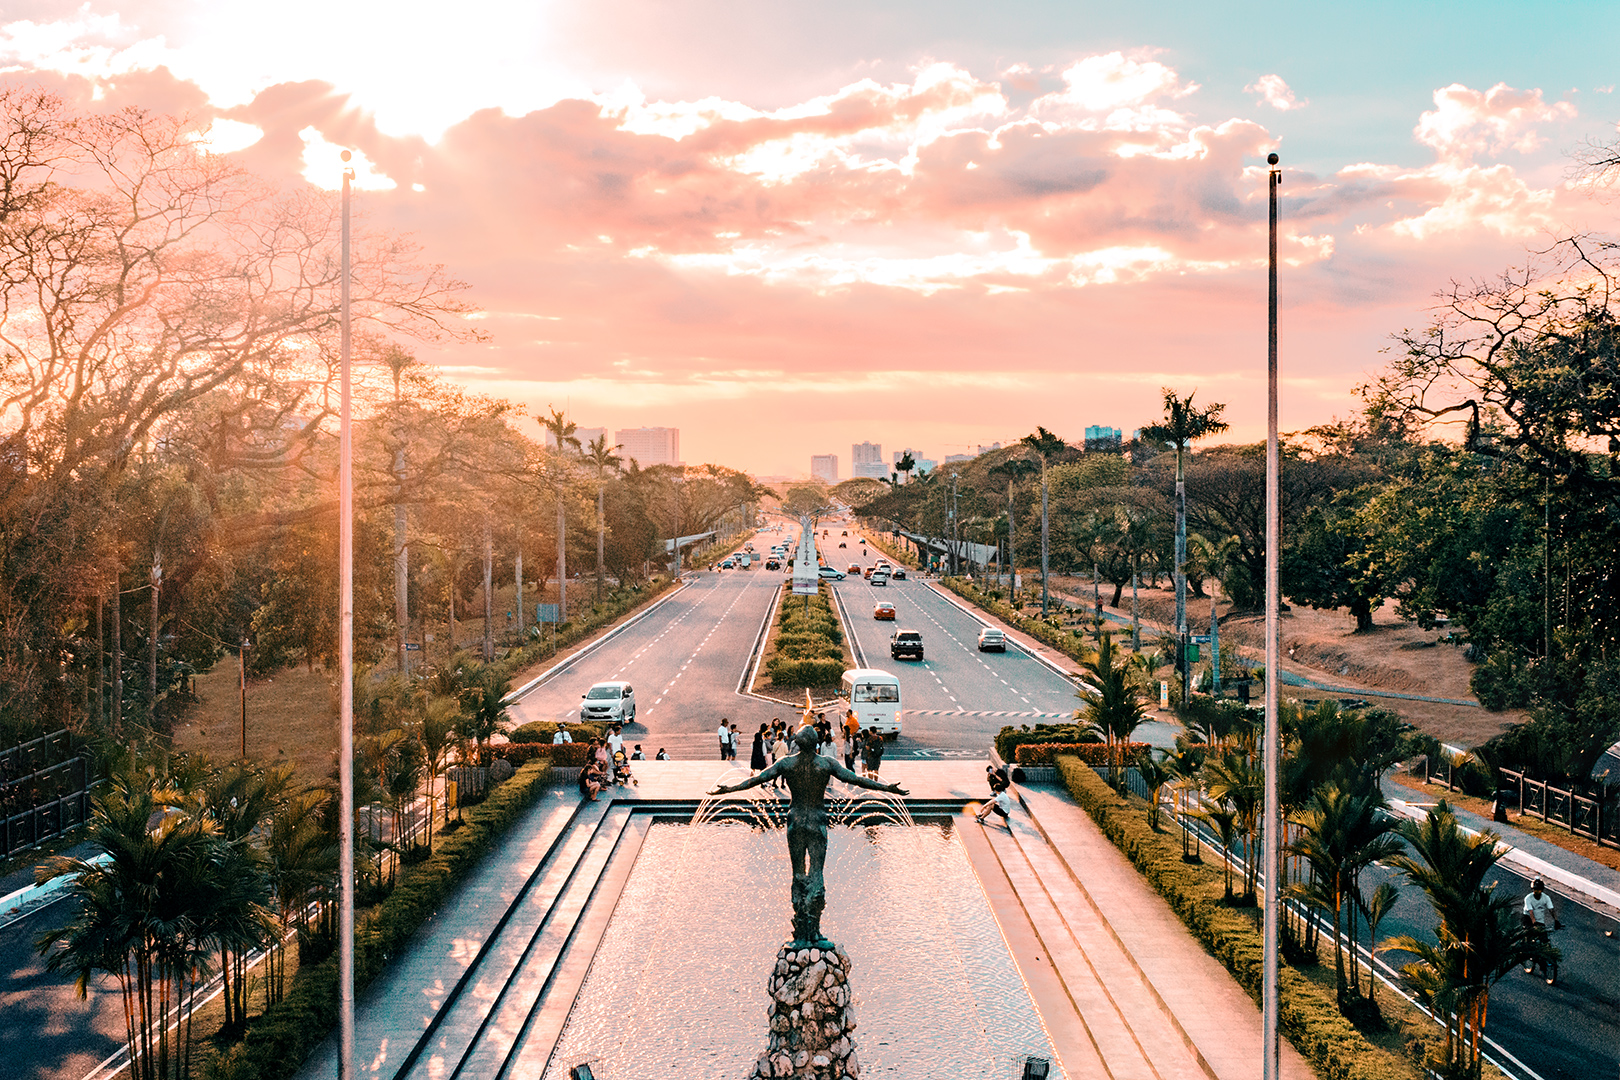
\includegraphics[width=\textwidth]{DSC_8805.jpg}
	\caption{Image used for comparison of file sizes.}
	\label{fig:hdr}
\end{figure}

\begin{figure}[htb]
	\centering
	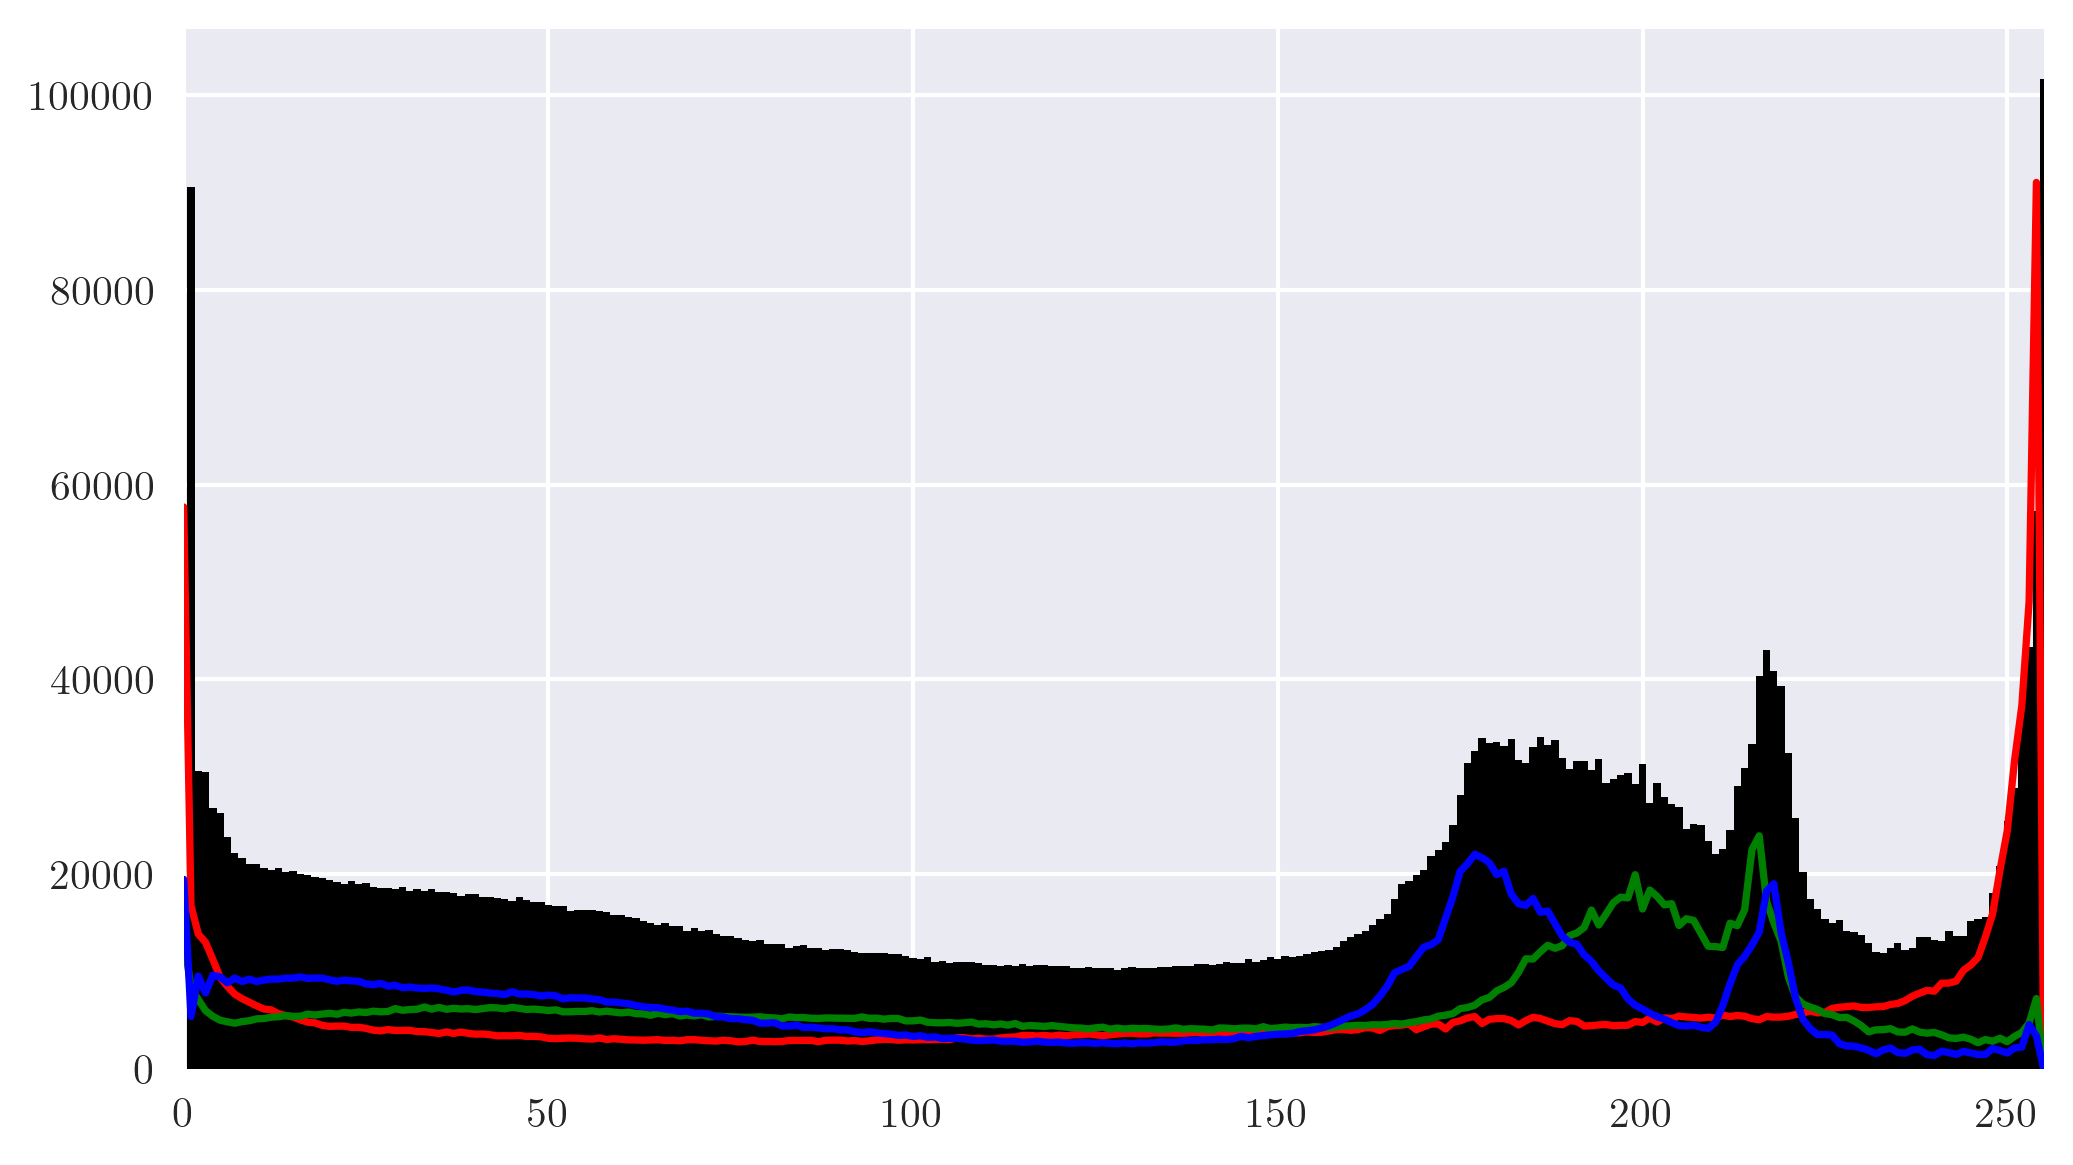
\includegraphics[width=\textwidth]{histogram.png}
	\caption{Red, green, blue, and gray histograms of Fig. \ref{fig:hdr}.}
	\label{fig:hist}
\end{figure}

In order to produce a binary image, I applied a threshold of 192 to Fig. \ref{fig:hdr}. The result is shown in Fig. \ref{fig:bin}.

\begin{figure}[htb]
	\centering
	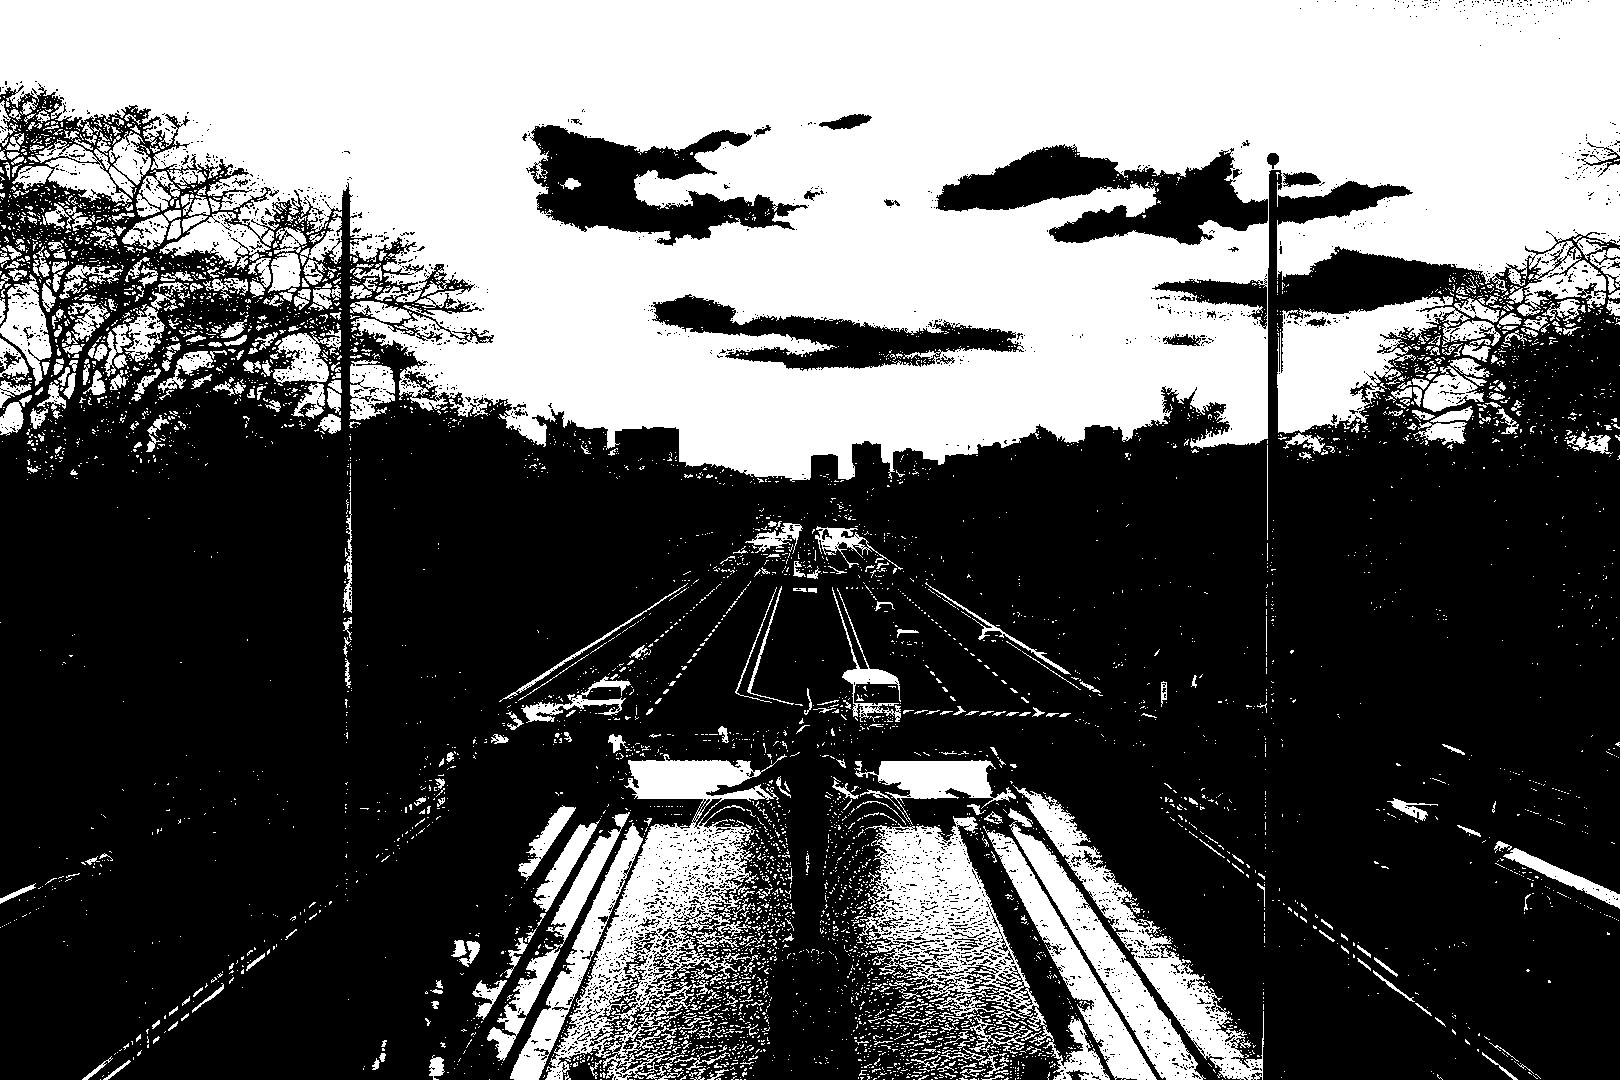
\includegraphics[width=\textwidth]{DSC_8805_bin.jpg}
	\caption{Fig. \ref{fig:hdr} saved as a binary image.}
	\label{fig:bin}
\end{figure}

\begin{table}[htb]
	\centering
	\caption{File sizes for various saved formats of Fig. \ref{fig:hdr}.}
	\label{tab:sizes}
	\begin{tabular}{|r|r|}
		\hline
		\textbf{Format} & \textbf{Size (KB)} \\ \hline \hline
		24-bit \texttt{JPG} & 1,474 \\ \hline
		16-bit \texttt{BMP} & 3,418 \\ \hline
		8-bit \texttt{PNG} & 3,240 \\ \hline
		8-bit \texttt{TIFF} & 1,053 \\ \hline
		8-bit \texttt{GIF} & 533 \\ \hline
		\texttt{JPG} (binary) & 391 \\ \hline
	\end{tabular}
\end{table}

In order to produce an indexed image, I first imported the image into Photoshop and set it to Index mode. I then extracted the 256 most common colors and saved them as a Photoshop Color Table (\texttt{.act}). I then applied this color indexing to the image and saved it one as a \texttt{TIFF} and one as a \texttt{GIF}. The result of the \texttt{TIFF} indexing along with its color table is shown in Fig. \ref{fig:tiff-indexed} and Table \ref{tab:indexed}, respectively. Notice that the ground portion of the image still looks decent because the boundaries of each color are considerably well-defined. However, the sky portion exhibits some visible degradation due to the smooth gradients in the original image. The \texttt{GIF} indexing in Fig. \ref{fig:gif-indexed} exhibits degradation even in the ground portion. I found out that this was due to the difference in the way the colors are sampled. In the former, the sampling of colors is locally adaptive, which allows transition of colors to be smoother, while in the latter, the sampling is uniform.

\begin{figure}[htb]
	\centering
	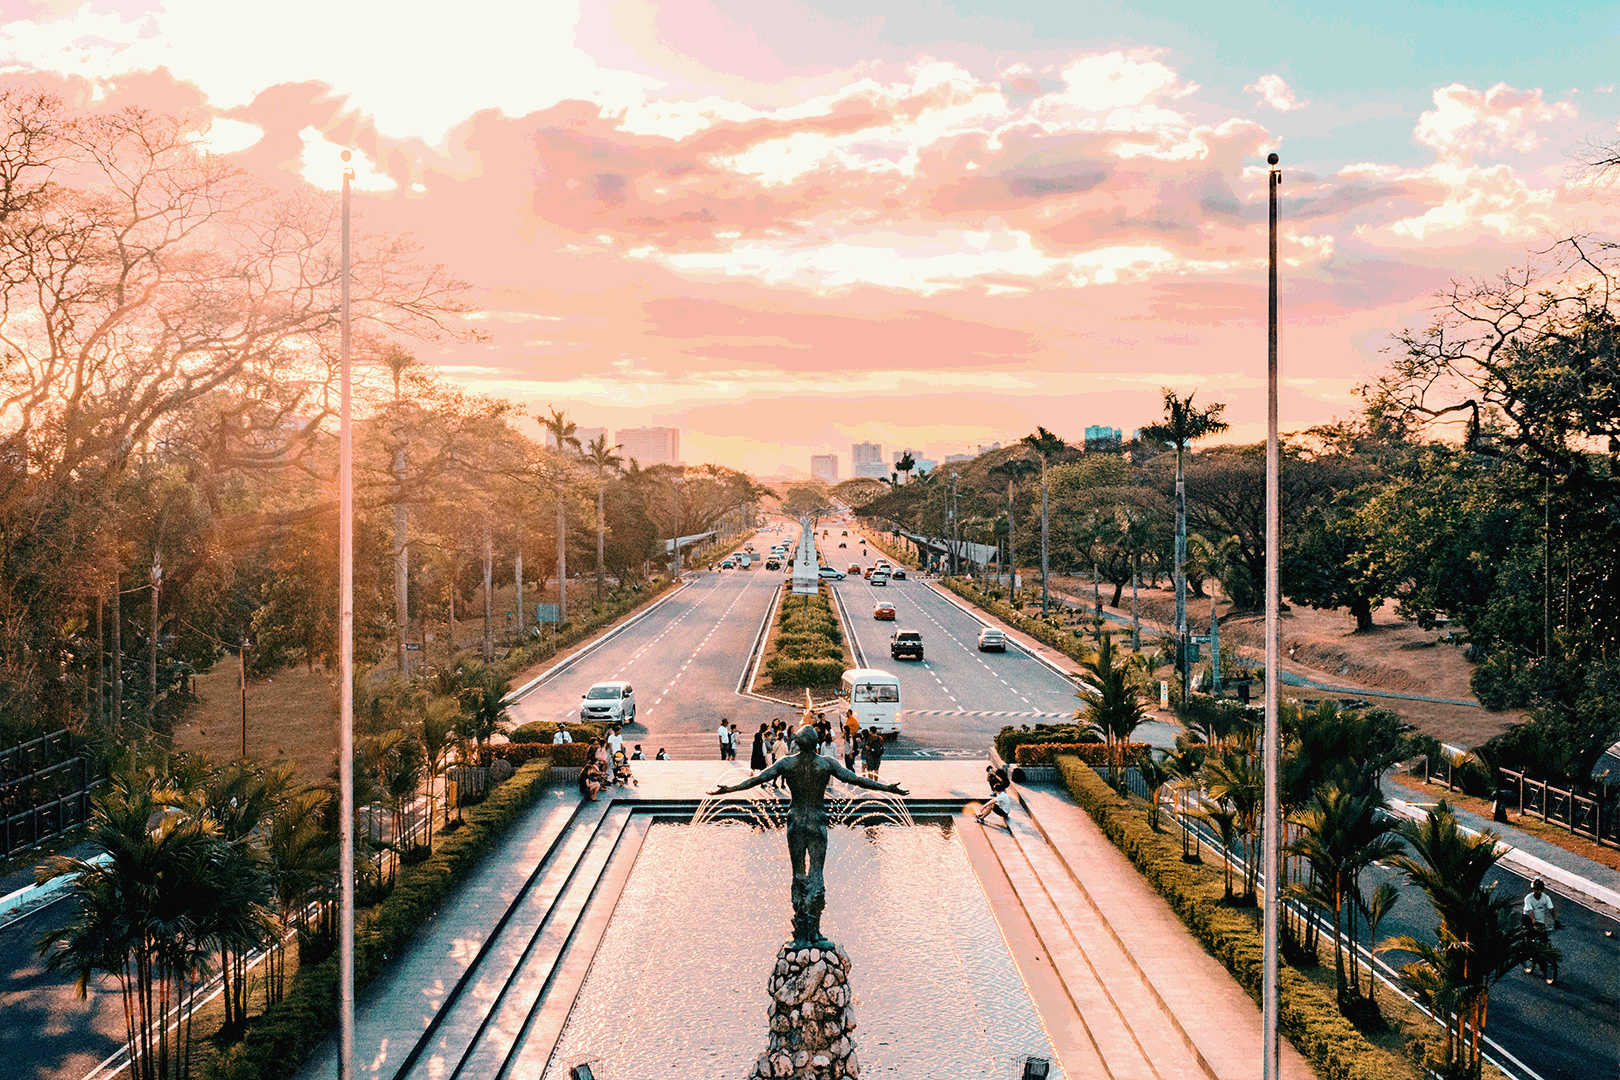
\includegraphics[width=\textwidth]{DSC_8805_tiff_indexed.png}
	\caption{Fig. \ref{fig:hdr} saved as a \texttt{TIFF} indexed image.}
	\label{fig:tiff-indexed}
\end{figure}

\begin{figure}[htb]
	\centering
	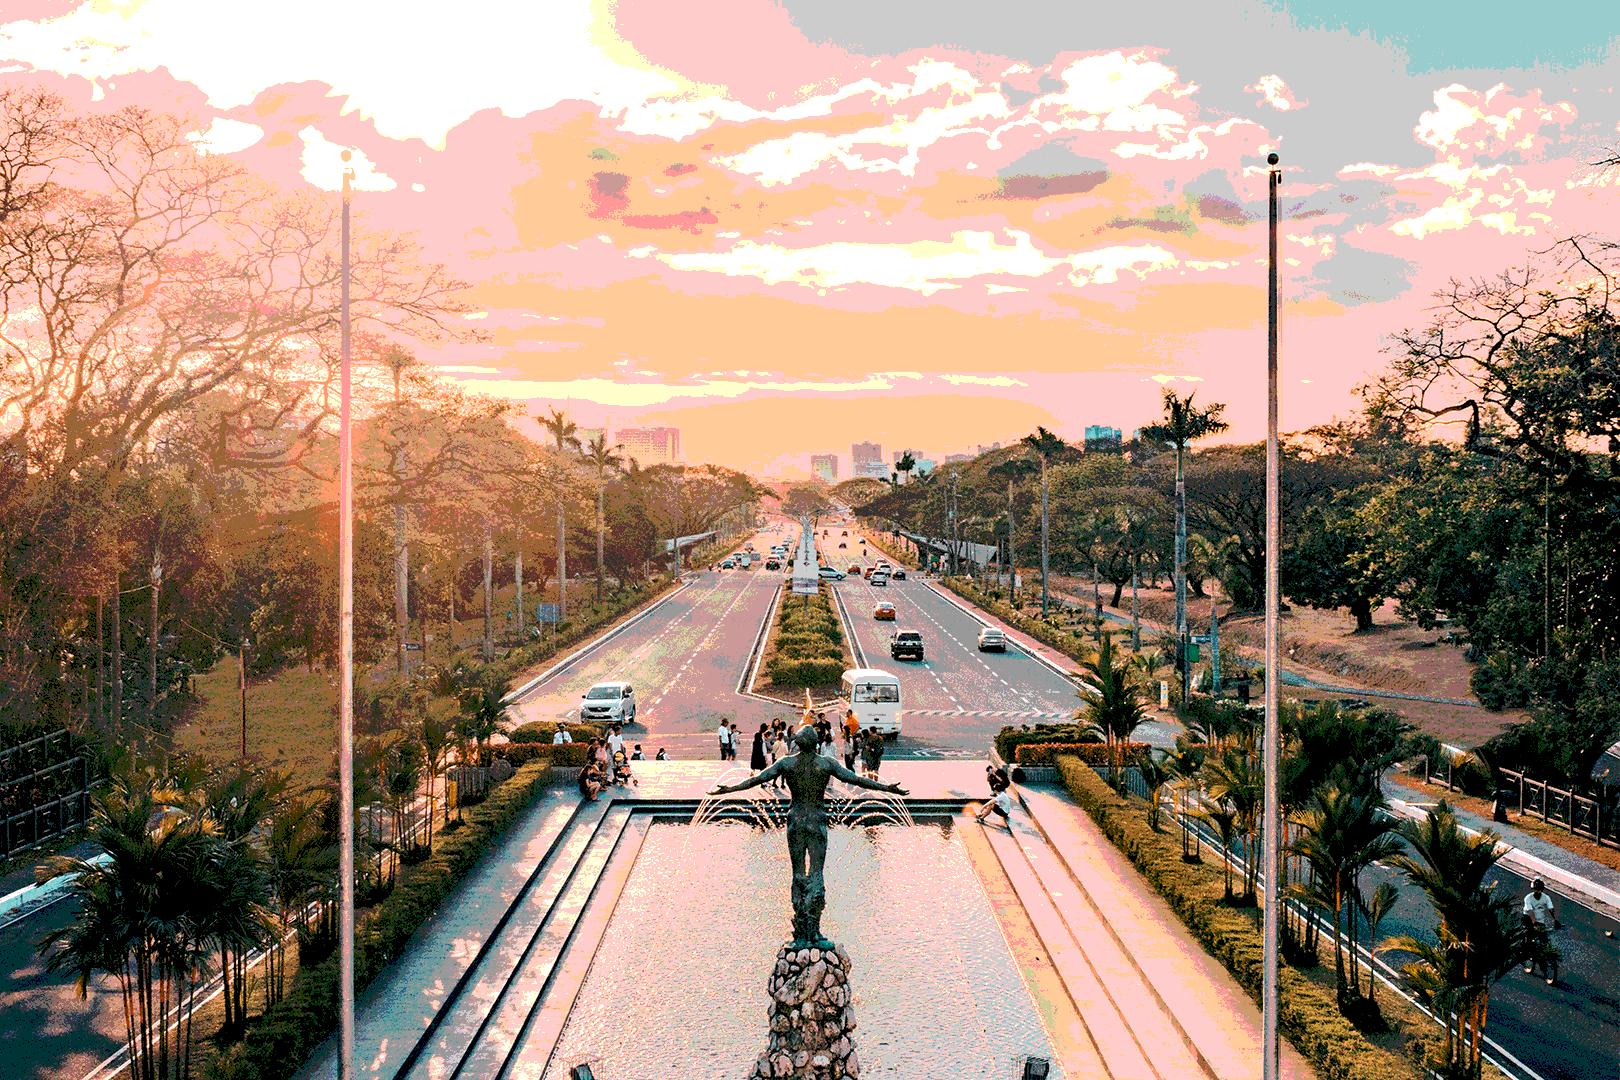
\includegraphics[width=\textwidth]{DSC_8805_gif_indexed.png}
	\caption{Fig. \ref{fig:hdr} saved as a \texttt{GIF} indexed image.}
	\label{fig:gif-indexed}
\end{figure}

\definecolor{index0}{rgb}{0.29,0.09,0.10}
\definecolor{index1}{rgb}{0.69,0.66,0.66}
\definecolor{index2}{rgb}{0.97,0.66,0.72}
\definecolor{index3}{rgb}{0.91,0.66,0.72}
\definecolor{index-2}{rgb}{0.03,0.03,0.03}
\definecolor{index-1}{rgb}{1,1,1}
\begin{table}[htb]
	\centering
	\caption{First and last few elements of the color table for Fig. \ref{fig:tiff-indexed}.}
	\label{tab:indexed}
	\begin{tabular}{|c|ccc|c|}
		\hline
		Index & R & G & B & Color \\ \hline \hline
		0 & 74 & 24 & 26 & \cellcolor{index0} \\ \hline
		1 & 177 & 168 & 169 & \cellcolor{index1} \\ \hline
		2 & 248 & 168 & 184 & \cellcolor{index2} \\ \hline
		3 & 232 & 168 & 184 & \cellcolor{index3} \\
		$\vdots$ & $\vdots$ & $\vdots$ & $\vdots$ & $\vdots$ \\
		254 & 7 & 7 & 7 & \cellcolor{index-2} \\ \hline
		255 & 255 & 255 & 255 & \cellcolor{index-1} \\ \hline
	\end{tabular}
\end{table}

\subsection{History}
Camera sensors are composed of arrays of light-sensitive detectors, and each component of these detectors have varying sensitivities and transfer functions which convert incident light into the red, green, and blue channels. In the \texttt{RAW} file format, the raw information captured by the sensor is stored without any compression or manipulation. This technology is still used at present especially by professional camera manufacturers---such as Nikon's \texttt{NEF} format and Canon's \texttt{CR2} format---in order to preserve all the information received by the camera's sensor, which provides an advantage when post-processing later on, especially when shooting in low light. As imaging technology developed, so has our ability to reproduce larger images. Eventually, storage capacity became an issue, which birthed the challenge of data compression.

One of the first formats to have taken up this challenge is the Graphics Interchange Format (\texttt{GIF}) in 1987 \cite{roelofs}. It uses the Lempel-Ziv-Welch (LZW) lossless compression algorithm, which provides up to 25\% compression. However, \texttt{GIF} is a pixel-dependent, 8-bit indexed format, so images could not show their full color range in this format. The file format quickly fell out of favor when its compression technique was patented in 1995 by Unisys Corporation \cite{wiggins}, who attempted to collect royalties from \texttt{GIF} users. Capitalism strikes again!

In the early 1990's, the International Organization for Standardization (ISO) and the International Telecommunication Union (ITU) formed a joint committee called the Joint Photographic Expert Group, the creator of the eponymous \texttt{JPEG} format. Its most common incarnation is the 24-bit version, which allocates 8 bits for each color channel, and its strength lies in its lossy discrete cosine transform (DCT)-based compression format to achieve up to 5\% compression. The way it is encoded allows the user to set the compression level desired, and for normal day-to-day usage, the data it discards is usually imperceptible.

In 1986, the Tagged Image File Format (\texttt{TIFF}) was developed by Microsoft and Aldus (now merged with Adobe), and takes its name due to its heavy dependence on tags, which relay the image information to the program accessing the file. It is highly versatile, supports a wide range of sizes, resolutions and color depths \cite{wiggins}, and can use LZW, ZIP, or other compression methods. However, its large file size as a consequence of its complexity limits its practical use.

In 1995, the Portable Network Graphics (\texttt{PNG}) format was created as the spiritual successor of \texttt{GIF} and hailed by some as the future of bit-mapped images \cite{wiggins}. Out of all the formats discussed here, it is probably the most flexible and allows for lossless compression, device-independent gamma correction, device-independent brightness consistency, transparency (now better-known as the alpha channel), redundant self-verification of data integrity, interlacing, and various pixel mapping schemes (indexed, grayscale, or true-color RGB).


\subsection{Programming basic imaging functions}
Some of the libraries that can be used for image processing in Python include the \texttt{matplotlib}, \texttt{opencv2}, and \texttt{PIL} modules. Some basic functions include:

\begin{itemize}
	\item \texttt{cv2.imread()}: reads an image from the computer and loads it as an $n$-dimensional \texttt{numpy} array.
	\item \texttt{matplotlib.pyplot.savefig()}: saves a valid \texttt{numpy} array as an image with the specified file format.
	\item \texttt{PIL.\_getexif()}: extracts the image metadata and stores it as a dictionary.
	\item \texttt{matplotlib.pyplot.hist()}: plots the histogram of an image.
	\item \texttt{cv2.COLOR\_RGB2GRAY}: converts an RGB image to grayscale; can be passed as an argument in \texttt{cv2.imread()}.
\end{itemize}


\begin{table}[!htb]
	\centering
	\caption{Self-evaluation.}
	\begin{tabular}{|r|c|}
		\hline
		Technical correctness & 5 \\ \hline
		Quality of presentation & 5 \\ \hline
		Initiative & 2 \\ \hline
		\textbf{TOTAL} & \textbf{12} \\ \hline
	\end{tabular}
	\label{tab:self-eval}
\end{table}


\bibliographystyle{spp-bst}
\bibliography{186-Act3}

\end{document}